\chapter{Specimen Request}
\label{chap:specimen-request}

A \emph{Request Center} can submit a request for a set of specimens, meeting a
criteria, to be shipped to one of it's locations.  The \entitytarget{Request}
aggregate in the specimen request module is used to manage this. Figure
\ref{fig:specimen-request} shows the model used by the aggregate.

\begin{figure}[H]
  \centering
  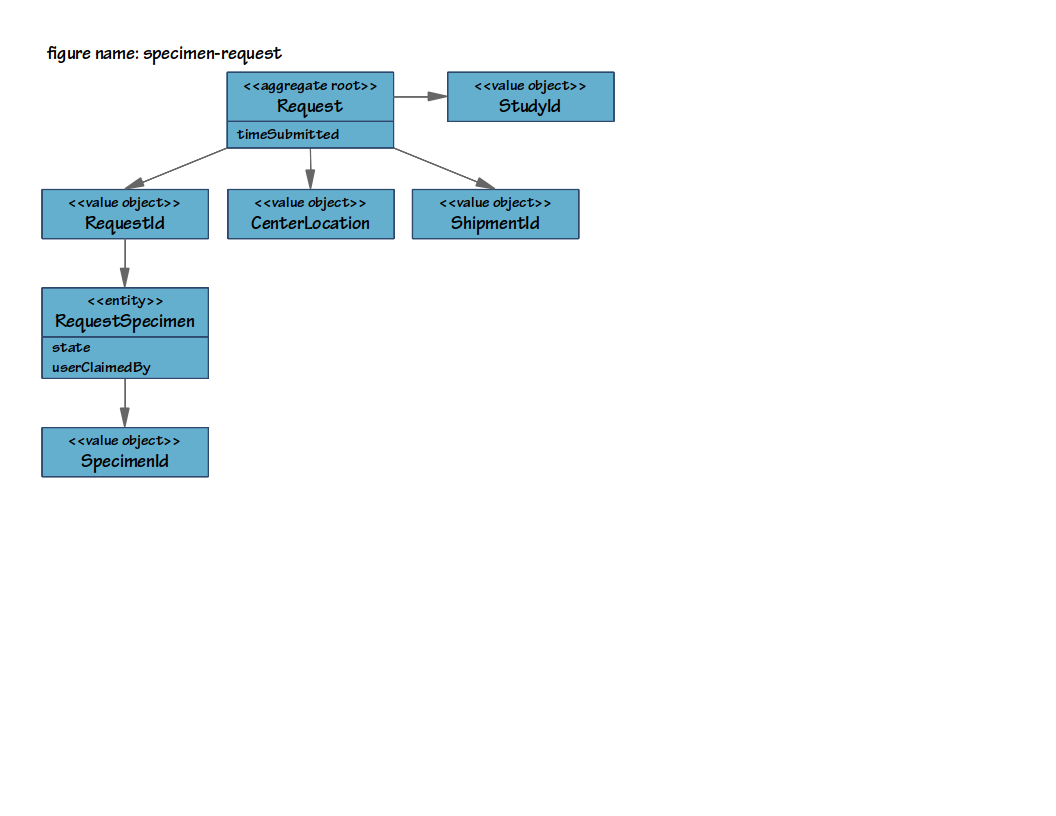
\includegraphics[trim={10mm 88mm 117mm 18mm}, clip,
    width=0.75\textwidth]{images/specimen-request}
  \caption{Specimen Request model}
  \label{fig:specimen-request}
\end{figure}

\subsection*{Request}
The \entitylink{Request} aggregate root has the following attributes:
\begin{itemize}
\item a unique ID to identify the request;
\item the time it was submitted;
\item the ID of the study the specimens are registered in;
\item the location of the centre where the package is to be shipped;
\item and the IDs of the shipments that contain the specimens.
\end{itemize}

It is possible that shipments from more than one storage centers is required to
fill the request.

\subsection*{RequestSpecimen}
A \entitytarget{RequestSpecimen} is created for each specimen that meets the
request criteria.

\vspace{10mm}

\emph{This section needs more work. It should be modelled more like a shopping
  cart application, where a user requests items, and then a technician fills the
  order and then ships it.}

% Local Variables:
% compile-command: "/usr/bin/rubber --pdf main"
% End:
